\chapter{Metodologia}
\label{cap:03}

Descrever metodologia, materiais e métodos utilizados no estudo, bem como os procedimentos experimentais realizados, nesta etapa será descrito vários assuntos sobre os passos a serem realizados iniciando com o levantamento dos dados, para uma analise e estudo posteriormente analisando todos os processos que são realizados, afim de iniciar o desenvolvimento.


\begin{figure}[ht]
\caption{Passos feito na plataforma miro}
\centering
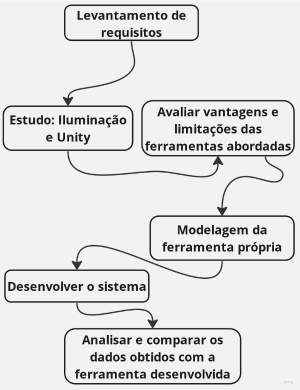
\includegraphics{imagens/Diagrama.jpg}

Fonte: Feito pelo autor
\label{fig:diagrama}
\end{figure}

\section{Levantamento de Requisitos}

Nessa sessão será abordado a pesquisa qualitativa feita a partir da ferramenta \textit{Relight} que usa de um algoritmo para identificação de camadas em uma imagem, assim, quando a imagem é colocada na ferramenta ela faz um mapeamento das áreas altas e baixas para criar as camadas, por esse motivo as camadas que são denominadas como mais alta recebe mais luz do que as mais baixas.

Porém a ferramenta tem uma funcionalidade a mais onde é possivel definir em que nível está a luz, fazendo com que a iluminação do objeto possa vir das camadas mais a baixo para as camadas acima, está ferramenta com a luz funciona como um pincel de adicionar em softwares de pintura, pois ela recebe a luz já existente na foto e complementa por cima com a luz própria, podendo ser de qualquer cor.

A seguir será mostrado na tabela, onde terá a avaliação qualitativa referente a vários tipos de imagens testadas a partir da ferramenta, que para efeitos deste trabalho serão utilizados os valores de alta resolução como acima de 720 pixels, média resolução entre 720 e 256 pixels e baixa resolução abaixo de 256 pixels, retratado na tabela:

Avaliação qualitativa da ferramenta

\begin{tabular}{l r r r}
Imagem & Alta Resolução & Média Resolução & Baixa Resolução\\
Objetos & Funciona  & Funciona  & Restrição\\
Humanos & Funciona  & Funciona  & Restrição\\
Paisagens & Funciona & Problema &  Problema\\
\end{tabular}

Nessa tabela, foi adotado três categorias para descrever o funcionamento: Funciona, Restrição e Problema.
A primeira categoria é utilizada para descrever que a imagem utiliza se comportou de forma correta, Restrição é a categorização para as imagens que funcionam mas em alguns casos ou áreas da imagem geram problemas, já a categoria Problema indica os casos onde a luz não reconhecia as formas de maneira correta.

\section{Estudo: Iluminação e Unity}
Nesse estudo será demonstrado algumas das partes que serão necessárias para o desenvolvimento da ferramenta, como a seguir que se iniciará com a iluminação nas histórias em quadrinhos.
Sempre que vemos uma cor clara e logo depois uma escura, isso significa que há um relevo muito grande ali, por exemplo  na Figura \ref{fig:batman}

\begin{figure}[ht]
\caption{História em quadrinhos, Batman}
\centering
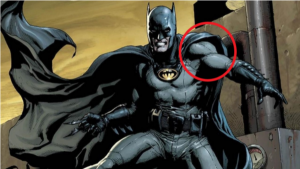
\includegraphics{imagens/batman.png}

Fonte: \cite{Bazela2022-yg}
\label{fig:batman}
\end{figure}    

Nesse quadrinho do Batman, podemos ver que em seu ombro está muito claro e logo acima onde sua capa está vem uma cor muito escura, isso nos mostra que a profundidade da capa é grande, ao ponto de não chegar nenhuma luz até ela, é claro que precisamos levar em consideração que nas HQ’s em geral os contrastes são muito maiores, porque traz esse volume nos trajes.

Partindo para o ramo da \textit{Unity} será preciso um aprendizado todo relacionado a iluminação dentro da ferramenta, uso dos objetos em cena e manipulação deles, pois para o desenvolvimento será necessário a criação de uma malha que forme a imagem, um sistema de camadas para que possa estabelecer profundidade, um sistema de alteração e manipulação da posição, cor e luminosidade do ponto de luz. E por fim um estudo básico de toda interface da \textit{Unity}.

Outro ponto importante no estudo, será a linguagem de programação \texttt{C\#} que é usada como alicerce para qualquer código que precise ser estruturado lá dentro, desde instanciar objetos dentro da cena até modificar configurações de câmera como movimento, posicionamento e angulo até para recebimento dos arquivos

\section{Avaliar vantagens e limitações das ferramentas abordadas}

O \textit{Relight} é uma ferramenta muito boa para processos de iluminação tanto para cenários como personagens, com uma boa modificação como profundidade, posição, cor e luminosidade, dando para o usuário a liberdade de dar personalidade as suas imagens.

Mas ainda existe várias limitações e elas que serão retratadas nessa seção, como foi visto na analise a cima na tabela é possível notar que quanto menor a imagem é, menos funcional ela passa a ser, por exemplo imagens em baixa resolução ou pixeladas começam a ter muitos problemas pois a luz não consegue distinguir os objetos na cena e muito menos paisagens pois com tantas cores perto uma das outras transforma a cena em uma desordem visual.

\section{Modelagem da ferramenta}

Uma malha deverá ser criada por cima de toda a imagem e definir um inteiro para a profundidade, cada \textit{pixel} dá imagem deve receber uma profundidade como pode se observar na Figura \ref{fig:sketch}

\FloatBarrier
\begin{figure}[ht]
\caption{Rascunho elaborado pelo autor}
\centering
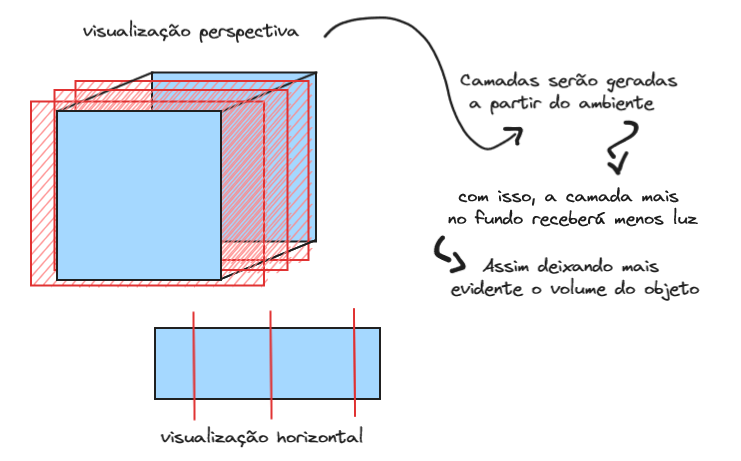
\includegraphics[scale=0.5]{imagens/Sketch.png}

\label{fig:sketch}
\end{figure}    
\FloatBarrier

Assim ele vai numerar toda a malha de \textit{pixels} na tela com números que podem ter uma variação maior dependendo do tamanho da imagem ( no caso de exemplo)

Será calculado de 1 a 9, mas com imagens imensas em alta resolução podemos pensar em usar de 1 a 100 ou até mais

Podemos pensar que dessa forma será possível utilizar essa profundidade para produzir uma luz pelas laterais ou pela frente e até atrás de elementos, sem perder sua funcionalidade até mesmo em imagens pequenas

Além disso, cada um desses valores definidos em cada \textit{pixel} da imagem, vão servir de referencia para criação de vários objetos, ele levará em consideração a distância e a variação de cor que foi atingida

Como por exemplo, se existir um objeto a frente da camada 1 até a 10 e um objeto atrás que está na camada 15, essa distancia de 5 camadas irá fazer o objeto dá frente se separar com o de trás transformando a cena com dois objetos ao invés de um


\section{Justificativa das Tecnologias a serem adotadas}

Será utilizado a IDE Visual Studio para a criação dos códigos que serão importados na \textit{Unity}, foi optado ele pois é o sistema mais robusto para a utilização do \texttt{C\#}.

Para o processo de desenvolvimento efetivo, além da IDE será usado a \textit{game engine}, Unity, que foi escolhida pela simplicidade em aplicar luz e criação de objetos bidimensionais em ambientes Tridimensionais, ou como é conhecido 2.5D, para assim poder criar com efetividade a malha e a luz aplicada a ela

\section{Avaliação Qualitativa}

Logo após todo o processo estiver concluído, chega a etapa da avaliação, nesse tópico irá apresentar como será feita a avaliação dos resultados obtidos a partir das analises feitas anteriormente, nesta comparação será possível avaliar os seguintes pontos, primeiramente a alteração em imagens de baixa resolução se é possível a partir desse novo algoritmo e se as vantagens irão se permanecer. Outro ponto que poderá ser analisado será a eficacia de executar a ferramenta e se ela é possível a partir dos cálculos necessários.